%
% __NOTE: (!) 
%      to build pdf with pdflatex you 
%      must do pdflatex --shell-escape PAVE_ISAV.tex 
%      because of minted import for code examples
%__
\documentclass[sigconf,authordraft]{acmart}%
\usepackage{minted}
%%
%% \BibTeX command to typeset BibTeX logo in the docs
\AtBeginDocument{%
  \providecommand\BibTeX{{%
    \normalfont B\kern-0.5em{\scshape i\kern-0.25em b}\kern-0.8em\TeX}}}

%%\setcopyright{acmcopyright}
%%\copyrightyear{2018}
%%\acmYear{2018}
%%\acmDOI{10.1145/1122445.1122456}

%% These commands are for a PROCEEDINGS abstract or paper.
%%\acmConference[Woodstock '18]{Woodstock '18: ACM Symposium on Neural
%%  Gaze Detection}{June 03--05, 2018}{Woodstock, NY}
%%\acmBooktitle{Woodstock '18: ACM Symposium on Neural Gaze Detection,
%%  June 03--05, 2018, Woodstock, NY}
%%\acmPrice{15.00}
%%\acmISBN{978-1-4503-9999-9/18/06}


%%
%% Submission ID.
%% Use this when submitting an article to a sponsored event. You'll
%% receive a unique submission ID from the organizers
%% of the event, and this ID should be used as the parameter to this command.
%%\acmSubmissionID{123-A56-BU3}

%%
%% The majority of ACM publications use numbered citations and
%% references.  The command \citestyle{authoryear} switches to the
%% "author year" style.
%%
%% If you are preparing content for an event
%% sponsored by ACM SIGGRAPH, you must use the "author year" style of
%% citations and references.
%% Uncommenting
%% the next command will enable that style.
%%\citestyle{acmauthoryear}

%%
%% end of the preamble, start of the body of the document source.
\begin{document}

%%
%% The "title" command has an optional parameter,
%% allowing the author to define a "short title" to be used in page headers.
\title{PAVE}

%%
%% The "author" command and its associated commands are used to define
%% the authors and their affiliations.
%% Of note is the shared affiliation of the first two authors, and the
%% "authornote" and "authornotemark" commands
%% used to denote shared contribution to the research.
\author{Samuel Leventhal}
\authornotemark[1]
%\authornote{Both authors contributed equally to this research.}
\email{samlev@cs.utah.edu}
\affiliation{%
  \institution{University of Utah School of Computing: Scientific Computing and Imaging Institute}
  %\streetaddress{P.O. Box 1212}
  %\city{Dublin}
  %\state{Ohio}
  %\postcode{43017-6221}
}
%\orcid{1234-5678-9012}
\author{Mark Kim}
\email{kimmb@ornl.gov}
\affiliation{%
  \institution{Oak Ridge National Lab}
  %\streetaddress{P.O. Box 1212}
  %\city{Dublin}
  %\state{Ohio}
  %\postcode{43017-6221}
}

\author{Dave Pugmire}
\email{pugmire@ornl.gov}
\affiliation{%
  \institution{Oak Ridge National Lab}}


%%
%% By default, the full list of authors will be used in the page
%% headers. Often, this list is too long, and will overlap
%% other information printed in the page headers. This command allows
%% the author to define a more concise list
%% of authors' names for this purpose.
\renewcommand{\shortauthors}{Leventhal and Kim, et al.}

%%
%% The abstract is a short summary of the work to be presented in the
%% article.
\begin{abstract}
 {\it In situ} deep learning for scientific visualisation has an increasingly broader venue for application as visualisation on large scale systems and machine learning techniques and applications continue to expand. In this work we offer an approachable platform for visualisation tasks by employing a neural network for real time rendering and accurate light transport simulation within the framework of Python, specifically PyTorch, made compatible for distributed systems and high performance computing (HPC). The provided model is a coalescence of VTK-m, a visualisation toolkit fit for massively threaded architectures, PyTorch, an  increasingly popular language within machine learning due to robust libraries for neural networks, and Adios2, an adaptable unified IO framework for data management at scale. The resulting work accomplishes this combination by utilising VTK-m to construct a path trace rendering tool able to fluidly and efficiently communicate to a conditional Generative Adversarial Network (cGAN) by means of Adios2 during training. The resulting generative model serves as a real-time filter for rendering images and visual simulations accurately approximating indirect illumination and soft shadows with quality comparable to offline approaches. 
\end{abstract}

%%
%% The code below is generated by the tool at http://dl.acm.org/ccs.cfm.
%% Please copy and paste the code instead of the example below.
%%

 \begin{CCSXML}
<ccs2012>
<concept>
<concept_id>10003752.10003753.10003761.10003762</concept_id>
<concept_desc>Theory of computation~Parallel computing models</concept_desc>
<concept_significance>500</concept_significance>
</concept>
<concept>
<concept_id>10003752.10003753.10003761.10003763</concept_id>
<concept_desc>Theory of computation~Distributed computing models</concept_desc>
<concept_significance>500</concept_significance>
</concept>
<concept>
<concept_id>10003752.10010070.10010071.10010085</concept_id>
<concept_desc>Theory of computation~Structured prediction</concept_desc>
<concept_significance>500</concept_significance>
</concept>
<concept>
<concept_id>10003752.10010070.10010071.10010261.10010276</concept_id>
<concept_desc>Theory of computation~Adversarial learning</concept_desc>
<concept_significance>500</concept_significance>
</concept>
<concept>
<concept_id>10003752.10010070.10010111.10011710</concept_id>
<concept_desc>Theory of computation~Data structures and algorithms for data management</concept_desc>
<concept_significance>500</concept_significance>
</concept>
<concept>
<concept_id>10003752.10003753.10003757</concept_id>
<concept_desc>Theory of computation~Probabilistic computation</concept_desc>
<concept_significance>300</concept_significance>
</concept>
<concept>
<concept_id>10003752.10010070.10010111.10010113</concept_id>
<concept_desc>Theory of computation~Database query languages (principles)</concept_desc>
<concept_significance>300</concept_significance>
</concept>
<concept>
<concept_id>10010405.10010432.10010439.10010440</concept_id>
<concept_desc>Applied computing~Computer-aided design</concept_desc>
<concept_significance>500</concept_significance>
</concept>
</ccs2012>
\end{CCSXML}

\ccsdesc[500]{Theory of computation~Parallel computing models}
\ccsdesc[500]{Theory of computation~Distributed computing models}
\ccsdesc[500]{Theory of computation~Structured prediction}
\ccsdesc[500]{Theory of computation~Adversarial learning}
\ccsdesc[500]{Theory of computation~Data structures and algorithms for data management}
\ccsdesc[300]{Theory of computation~Probabilistic computation}
\ccsdesc[300]{Theory of computation~Database query languages (principles)}
\ccsdesc[500]{Applied computing~Computer-aided design}

%%
%% Keywords. The author(s) should pick words that accurately describe
%% the work being presented. Separate the keywords with commas.
\keywords{VTKm, neural networks, generative adversarial network, Adios, PyTorch, path tracing}

%% A "teaser" image appears between the author and affiliation
%% information and the body of the document, and typically spans the
%% page.
\begin{teaserfigure}
  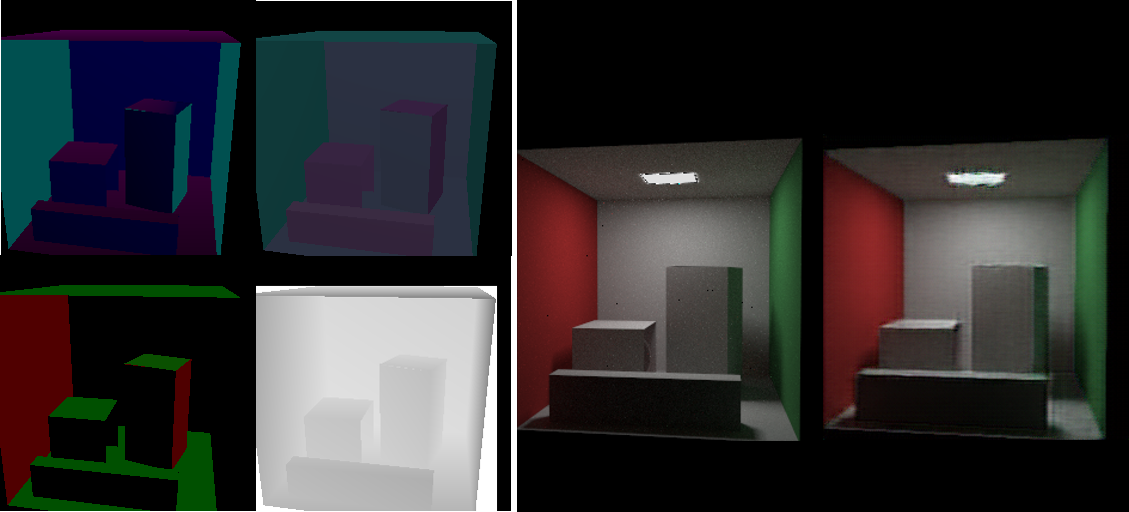
\includegraphics[width=\textwidth]{buffer_results_teaser.png}
  \caption{\textmd{Rendered Conditional Geometry Buffers ({\bf left set}) and artificial rendering with conditional generative adversarial neural network ({\bf right couple}) comparing ground truth path traced rendering ({\bf left}) with image generated ({\bf right}).}}
  \Description{Conditional Buffers and path traced rendered with VTKm to be used for training a PyTorch conditional generative adversarial network.}
  \label{teaser}
\end{teaserfigure}

%%
%% This command processes the author and affiliation and title
%% information and builds the first part of the formatted document.
\maketitle
\section{Applicable ``Area of Interests'' Targets}
{\footnotesize
\begin{enumerate}
    \item In situ data management and infrastructures
Current Systems: production quality, research prototypes , Opportunities ,Gaps

Current Systems: integration of VTKm, Adios2 and Python (PyTorch). Prototype being a conditional generative adversarial network (cGAN) designed to use a VTKm based pathtracer applied but not limited to learning global illumination and light behavior in rendering tasks. 
Opportunities: Introducing a framework allowing researchers easy access to python on HPC systems as well as machine learning aided technique to treat and study experimental data used in scientific simulations as learnable probability distributions with derived conditional dependencies of interest.

   \item System resources, hardware, and emerging architectures.
Enabling Hardware, Hardware and architectures that provide opportunities for In situ processing, such as burst buffers, staging computations on I/O nodes, sharing cores within a node for both simulation and in situ processing

Enabling Hardware: By constructing an architecture allowing for Python to interface with VTKm data management controlled by Adios2 the proposed software allows for a well distributed simulation task among cores.

  \item Methods and algorithms:
Analysis: feature detection, statistical methods, temporal methods, geometric and topological methods 
Visualization: information visualization, scientific visualization, time-varying methods
  \item Case Studies and Data Sources
In situ methods/systems applied to data from simulations and/or experiments / observations
  \item Simulation and Workflows:
Integration:data modeling, software-engineering, 
Workflows for supporting complex in situ processing pipelines
  \item Requirements, Usability:
Reproducibility, provenance and metadata

\end{enumerate}
}

\section{Introduction}


\section{Related Work}

Real time true to life quality renderings of light transport remains an active area of research with a number of various approaches. To preserve real-time rates, previous works have stored precomputed radiance transfers for light transport as spherical functions within a fixed scene geometry which are then adjusted for varied light and camera perspective through projections within a basis of spherical harmonics \cite{sloanPrecompRad}. Similarly, Light Propagation Volumes have been used to iteratively propagate light between consecutive grid positions to emulate single-bounce indirect illumination \cite{kaplanyanCasac}. More recently, deep neural  networks have been employed as a learned look up table for real-time rates with offline quality. With the use of convolutional neural networks Deep Shading is able to translate screen space buffers to into desired screen space effects such as indirect light, depth or motion blur. Similar to the methodology implemented in this work, Deep Illumination uses a conditional adversarial network (cGAN) to train a generative network with screen space buffers allowing for a trained network able to produce accurate global illumination with real-time rates at offline quality through a ``one network for one scene'' setting  \cite{deepillum}.

\section{Technique Overview}

Utilisation of PAVE consists of three consecutive phases: rendering phase of conditional training images, training phase of the generative neural network, and execution phase of the trained network. Three core components, VTK-m, PyTorch, and Adios2 fufill a unique functional requirement during each stage. In this section we describe the independent design and global role each system plays.

\subsection{System Overview}
 
To achieve our goal of a conditional generative neural network capable of rendering geometric dependent object path simulations we begin by rendering informative conditional image buffers along with ground truth scene renderings. For this purpose the VTK-m was chosen due to its scalability and robust capability for HPC visualisation tasks. Provided the training set of conditional and ground truth images two neural networks, one convolutional and one generative, play a zero-sum game common to training GANs. To segue data management of training images the path tracer saves the training set in a distributed setting with the use of Adios2. During training PyTorch is then able to retrieve needed image data through the use of the adaptable IO provided by Adios's Python high-level APIs.

\subsection{Path Tracer Design}

Conditional image attributes and high quality ground truth rendered images are required for the training stage. For this reason the first stage of PAVE consists of generating a visual scene or simulation with VTK-m. Within the framework of VTK-m the implemented ray tracer renders images through means common to commercial ray tracers such as Monte Carlo sampling for shapes of interest, light scattering, randomly directed light paths, material sampling and direct sampling. The image buffers needed to compute light paths afford an informative conditional dependence on the behavior of lighting based on the geometry and light sources within a scene. These conditional buffers, namely albedo, direct lighting, normals of surfaces and depth with respect to camera are then stored within VTK-m with Adios to maintain scalability of the system. For subsequent phases of PAVE the training data can then be retrieved from file again through Adios differing only in the API needed. 

\subsection{Neural Network Design}

The cGAN used closely follows that introduced by Thomas and Forbes with Deep Illumination \cite{deepillum}. Both the discriminator and generator network are deep convolutional neural networks implemented in PyTorch using training data retrieved from Adios files formatted and stored by the VTK-m path tracer. The training stage relies on four conditional buffers depth, albedo, normals and direct lighting along with an associated ground truth image of high light sample count and ray depth. Given the four conditional buffers the generator attempts to construct the ground truth image from noise. The discriminator is then fed both the generated and ground truth image. The loss used for the gradient back propagation update of both networks is based on the quality of the discriminators ability to classify the artificial and true image in which the generator is greater penalised when the discriminator accurately differentiates the two images, and similarly, the discriminator has a larger loss when incorrectly identifying real from fabricated images. The generator is then considered to have converged when the discriminator predicts both generated and true images with equal probability. For both discriminator and generator networks the activation functions used between layers is LeakyReLu and Sigmoid for the final layer \cite{maasLeaky}. Batch normalisation is also performed between internal layers to minimise covariant shift of weight updates and improve learning for the deeper networks used \cite{ioffeBatch}.

\subsubsection{Discriminator Network}

For discriminating between artificial and ground truth image renderings a deep convolutional patchGAN network is used motivated by the added advantage of providing a patch-wise probability of an image in question as being real or fake. The benefit of a patch-wise probability allows for higher regional accuracy within an image as well as applicable for image-to-image tasks as introduced by Isola et. al. \cite{isolaPatch}. 

As input during training the discriminator network is given the set of conditional space buffers along with either the visualisation generated by the cGAN generator network or the ground truth global illumination rendering produced with the VTK-m path tracer. Taking into account the conditional buffers the discriminator attempts to provide the rendered image as artificial, e.g. generated by the adversarial network, or real. Based on the performance of the discriminator the loss is computed using the classic loss for GAN training along with an L1 loss in order to not only produce original content but to also preserve structure and light information \cite{isolaL1}. Training is complete, and the generator has converged, when the discriminator predicts real from fake images with a 50-50 percent chance. At this point the discriminator network is discarded and the resulting generator affords a real-time visualisation tool able to produce accurate global illumination given conditional geometric buffers.

\subsubsection{Generator Network}

The generative network used is a deep convolutional network consisting of an encoder and decoder with skip connections concatenating equal depth layers of the encoding and decoding stages. Due to the illustrative `shape' of this design the network is denoted a U-Net as introduced by Ronneberger et. al. for medical segmentation \cite{ronnebergerUnet}. The motivation for utilising a U-Net is due to success of the skip connections linking the decoded convolutional process to the encoded upconvolutional in capturing geometric and spatial attributes. The generator retrieves as input through Adios global illumination buffers saved to file once rendered with VTK-m. 

\subsection{Core Design Pattern}

For our PyTorch in situ proposal the current systems we employ are VTK-m, for rendering path traced images and conditional geometry buffers focus, and Adios2 for data management. We discuss the design pattern for our in situ visualisation task with support from deep learning in the order of operations followed within the pipeline of use. Namely, we present the design pattern for rendering light transport in VTK-m coupled with data transport to PyTorch (\ref{pathtracer}). Subsequently we explain the infrastructure for embedding VTK-m throughput managed by Adios2 within PyTorch and demonstrate through example (\ref{pytorch}) by  instantiating a PyTorch data interface allowing for data parallelization and multi-GPU/distributed training as used within the framework for training our cGAN model. 

\subsubsection{VTK-m Data Generation and Adios2 Data Transport}\label{pathtracer}

Path traced images are maintained within C++11 as VTK-m arrays which can be passed by reference directly to PyTorch using Adios2 APIs or written to Adios2 .bp file and later retrieved during the data loading step when training or utilising the neural network to generate novel scene renderings from geometry buffers. 

\subsubsection{PyTorch Design}\label{pytorch}

For training, our solution used by the cGAN is ``{\it AdiosDataLoader}'', a data class inheriting from the abstract indexing class PyTorch {\it torch.utils.data.Dataset}. The {\it AdiosDataLoader} employs Adios2 to either retrieve from file or have passed by reference vector representations of path traced images and conditional buffers. Within VTK-m during generation these vectors represented as VTK-m vectors and within PyTorch as numpy arrays. In this manner the training or test sets needed by PyTorch and created by VTK-m are available to PyTorch in situ or with reference to written memory. If retrieving VTK-m's renderings PyTorch will compile Adios2 attributes from file as tabled by Adios2 into .bp files. VTK-m generated datasets can be retrieved with {\it read\_adios\_bp()} or passed to a similar {\it get\_adios\_bp()} and subsequently forwarded to our {\it get\_split()}  to partition the dataset into 60\% training, 20\% testing and 20\% validation subsets. The split datasets are then used to construct the {\it AdiosDataLoader} class which inherits from the {\it torch.utils.data.DataLoader} thereby providing a data sampler of our VTK-m renderings with a single-process or multi-process iterator over the dataset affording the tools necessary to train our neural networks in the canonical manner.

% other example scripts
%\inputminted{python}{pytorchAdiosRead.py}
%\inputminted{python}{trainingSplit.py}

\noindent\rule{0.5\textwidth}{1pt}
\inputminted{python}{pytorchDataLoader.py}
%\inputminted{python}{adiosdataloader.py}
\noindent\rule{0.5\textwidth}{1pt}

In the above code sample the {\it AdiosDataLoader} class is used to partition the data set into training, validation and testing as well as offer a distributable data sampler with an array-like data structure allowing index access to elements and collection size functionality.

\noindent\rule{0.5\textwidth}{1pt}
\inputminted{python}{adiosdataloader.py}
\noindent\rule{0.5\textwidth}{1pt}

\section{Cornell Box Experiment}

To evaluate the quality of in situ deep learning aided visualisations train the cGAN networks on rendered images of a Cornell box, a commonly used 3D modelling framework for quality assessment. We train the model using renderings of the Cornell box with high light sample count and depth computation per ray for various camera angle perspectives into the box along with the associated image geometry buffers for a given camera orientation. We then assess the quality of the models final generated renderings looking at the accuracy of global illumination. We then also demonstrate the performance of the models ability to render global illumination when given image buffers for a novel scene not used for training similar in content but not exact. The scene used for training is comprised of the classic set up with one overhead light source in the center of a white ceiling, a white back wall and a white floor. The remaining walls are then colored red on the left and green on the right in order to afford different colored light transport and demonstrate diffuse interreflection. The contents of the Cornell box are three cuboids of various shapes and sizes to provide diverse shading and diffused lighting. 

%\vspace{-1.5em}
\begin{figure}[h]
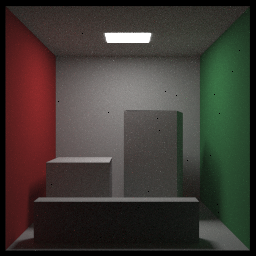
\includegraphics[width=0.25\textwidth]{sc-1080-d-45.png}
\end{figure}
%\vspace{-1em}

The conditional differed shading geometry buffers used are direct lighting, normal planes, depth and albedo as shown in figure \ref{teaser}.
\iffalse
\begin{figure}[h]
\caption{\textmd{Global illumination conditional image buffers. {\bf Top:} Albedo, left. Depth, right. {\bf Bottom:} Normals, left. Direct lighting, right.}}
\includegraphics[width=0.40\textwidth]{demo.png}
\label{Gbuf}
\end{figure}
\fi
The geometry buffers serve as joint variables for the conditional probability distribution which the global illumination path traced images are considered to exist. The conditional arguments in this experiment then aid the cGAN in learning behavior of light paths given the geometry of a scene in question. 

\section{Results}
\subsection{Cornell Box Experiment Results}
The resulting generated images show promising results for deep learning aided in situ scientific visualisation. We observe the network successfully learned to emulate light transport in a realistic fashion with offline performance {\bf EXAMPLE}. What is more, though designed in a ``one network for one scene'' setting, the generative net proved to be adaptive and able to generate accurate renderings for not only unobserved camera orientation renderings during training but also varied scenes of a similar flavor when provided the conditional geometry buffers of the novel scene. 

\subsection{Solution Design Assessment}

To render \_\_\_ 256x256 images with VTK-m on 2 \_\_\_\_ GPUs required \_\_\_ hours. Training the cGAN on this image data set over \_\_\_ epochs on the same machine took \_\_\_ hours. Once trained the run time of applying the generative U-Net provided the conditional buffer set averages \_\_\_ seconds. 

\section{Conclusions}



%%
%% The acknowledgments section is defined using the "acks" environment
%% (and NOT an unnumbered section). This ensures the proper
%% identification of the section in the article metadata, and the
%% consistent spelling of the heading.
\begin{acks}
Identification of funding sources and other support, and thanks to
individuals and groups that assisted in the research and the
preparation of the work should be included in an acknowledgment
section, which is placed just before the reference section in your
document.
\end{acks}

%%
%% The next two lines define the bibliography style to be used, and
%% the bibliography file.
\bibliographystyle{ACM-Reference-Format}
\bibliography{pave_ref}

%%
%% If your work has an appendix, this is the place to put it.
%\appendix
%\section{Appendix}



\end{document}
\endinput
%%
%% End of file `sample-authordraft.tex'.
